\section{Dimensions}
\label{sec:forward_dimensions}
{\small
\begin{center}
\begin{longtable}{| p{1.2in} || p{1.0in} | p{4.0in} |}
	\hline 
	{\bf Name} & {\bf Units} & {\bf Description} \endfirsthead
	\hline 
	{\bf Name} & {\bf Units} & {\bf Description} (Continued) \endhead
	\hline 
	\hline 
	nCells & $unitless$ & The number of polygons in the primary grid. \\ 
	\hline
	nEdges & $unitless$ & The number of edge midpoints in either the primary or dual grid. \\ 
	\hline
	maxEdges & $unitless$ & The largest number of edges any polygon within the grid has. \\ 
	\hline
	maxEdges2 & $unitless$ & Two times the largest number of edges any polygon within the grid has. \\ 
	\hline
	nVertices & $unitless$ & The total number of cells in the dual grid. Also the number of corners in the primary grid. \\ 
	\hline
	TWO & $unitless$ & The number two as a dimension. \\ 
	\hline
	R3 & $unitless$ & The number three as a dimension. \\ 
	\hline
	vertexDegree & $unitless$ & The number of cells or edges touching each vertex. \\ 
	\hline
	nVertLevels & $unitless$ & The number of levels in the vertical direction. All vertical levels share the same horizontal locations. \\ 
	\hline
	nVertLevelsP1 & $unitless$ & The number of interfaces in the vertical direction. \\ 
	\hline
\end{longtable}
\end{center}
}
\section[Namelist options]{\hyperref[chap:namelist_sections]{Namelist options}}
\label{sec:forward_namelist_tables}
Embedded links point to more detailed namelist information in the appendix.
\subsection[velocity\_solver]{velocity\_solver}
\label{subsec:forward_nm_tab_velocity_solver}
\section{Velocity Solver}
\label{sec:velocity_solver}

\subsection{Overview}

MPAS-Seaice uses a `B' Arakawa type grid \citep{Arakawa77} with both components of velocity defined at cell vertices and sea-ice concentration, volume and other tracers defined at cell centers (see Chapter \ref{chap:mpas_grid_description}). When using CICE-like quadrilateral meshes, this allows the velocity solver algorithm of MPAS-Seaice to reduce to that of CICE, allowing CICE and MPAS-Seaice to use identical test cases and allow rapid testing and development. 

In CICE the velocity components are aligned with the quadrilateral mesh. This is not possible, in general, with MPAS-Seaice since a SCVT MPAS mesh does not have edges with perpendicular directions as in a quadrilateral mesh. Instead, the velocity components at a given MPAS vertex are defined as eastwards ($u$) and northwards ($v$), irrespective of the orientation of edges joining that vertex. Such a definition, however, would result in a convergence of $v$ components at the geographic North Pole and strong metric terms in the velocity solution. Consequently, in addition, we rotate these definitions of $u$ and $v$ so that their pole lies on the geographical equator at $0^\circ$ longitude. 

To prognose sea-ice velocity we solve the same sea-ice momentum equation as CICE \citep{Hibler79,Hunke97}:
\begin{equation}
m \frac{\partial{\boldsymbol{u}}}{\partial{t}} = \boldsymbol{\nabla} \cdot \boldsymbol{\sigma} + \boldsymbol{\tau_a} + \boldsymbol{\tau_w} - \boldsymbol{\hat{k}} \times m f \boldsymbol{u} -mg \boldsymbol{\nabla}H_o.
\end{equation}
Here $m$ is the mass of snow and ice per unit area, $\boldsymbol{u}$ is the sea-ice velocity, $\boldsymbol{\sigma}$ is the ice internal stress tensor, $\boldsymbol{\tau_a}$ and $\boldsymbol{\tau_w}$ are the horizontal stresses due to atmospheric winds and ocean currents respectively, $\boldsymbol{\hat{k}}$ is the unit vector normal to the Earth surface, $f$ is the Coriolis parameter, $g$ is the acceleration due to gravity and $H_o$ is the ocean surface height. The second to last term represents the Coriolis force and the last term represents the force due to the ocean surface tilt. Only the divergence of internal stress and ocean surface tilt terms depend on horizontal differential operators. During coupled simulations the ocean model provides the ocean surface tilt term, whereas in non-coupled simulations we assume that the ocean currents are in geostrophic balance so that
\begin{equation}
mg \boldsymbol{\nabla}H_o = m f \boldsymbol{\hat{k}} \times \boldsymbol{u_o}
\end{equation}
where $\boldsymbol{u_o}$ is the ocean surface velocity. Consequently, only the divergence of internal stress depends on the properties of the horizontal grid employed, and only adaptations to this stress term are required to adapt the velocity solver of CICE to MPAS meshes. The other terms in the momentum equation are solved in an identical way to CICE.

Determination of the divergence of the internal stress can be broken down into three stages: 
\begin{enumerate}
\item The strain rate tensor is determined from the velocity field.
\item The stress tensor at a point is determined, through a constitutive relation, from the strain rate tensor at that point.
\item The divergence of this stress tensor is calculated. 
\end{enumerate}
As in CICE we use an Elastic-Viscous-Plastic (EVP) rheology \citep{Hunke97} for the constitutive relation. This step does not depend on the details of the horizontal mesh and we use the same formulation as CICE. We develop two schemes to calculate the strain rate tensor and the divergence of internal stress on MPAS meshes. A variational scheme is based on that used in CICE \citep{Hunke02}, whereas a weak scheme uses the line integral forms of the symmetric gradient and divergence operators. These schemes are described in the following sections.

\subsection{Variational Scheme}

We develop a variational scheme for calculating the divergence of stress based on that of \citet{Hunke02} but adapted for arbitrarily shaped and sided convex polygons. This scheme is based on the fact that over the entire domain, $\Omega$, and ignoring boundary effects, the total work done by the internal stress is equal to the dissipation of mechanical energy:
\begin{equation}
\int_\Omega \boldsymbol{u} \cdot (\boldsymbol{\nabla} \cdot \boldsymbol{\sigma}) \mathrm{d}A = -\int_\Omega (\boldsymbol{\sigma_{11}} \boldsymbol{\dot{\epsilon}_{11}}  + 2 \boldsymbol{\sigma_{12}} \boldsymbol{\dot{\epsilon}_{12}} + \boldsymbol{\sigma_{22}} \boldsymbol{\dot{\epsilon}_{22}}) \mathrm{d}A.
\label{eqn:work_done}
\end{equation}
Here $\boldsymbol{\dot{\epsilon}}$ is the strain rate tensor and the integrals are area integrals over the whole model domain. The work done over the whole domain can be split into a sum over the contribution to the work done from each cell on the dual Delaunay mesh. Each dual cell on the dual mesh consists of a triangle surrounding a single vertex point where the discretized velocity is defined. Equation \ref{eqn:work_done} can then be written as
\begin{equation}
\sum_i^{n_d} \int_i \boldsymbol{u} \cdot (\boldsymbol{\nabla} \cdot \boldsymbol{\sigma}) \mathrm{d}A = D(u_1, u_2, ..., u_n, v_1, v_2, ..., v_{n_d})
\end{equation}
where the left-side sum is over the $n_d$ cells of the dual mesh, the integral is an area integral over each dual cell,  and the dissipation of mechanical energy has been written as a function of the discretized velocity components.
Writing the two components of the divergence of stress as $F_u=(\nabla \cdot \sigma)_u$ and $F_v=(\nabla \cdot \sigma)_v$, then
\begin{equation}
\sum_i^{n_d} \int_i (uF_u + vF_v) \mathrm{d}A = D(u_1, u_2, ..., u_n, v_1, v_2, ..., v_{n_d}).
\end{equation}
If we assume that within the dual cell the velocity is constant, it follows that
\begin{equation}
\sum_i^{n_d} (u_i F_{ui} + v_i F_{vi}) A_{ui} = D(u_1, u_2, ..., u_n, v_1, v_2, ..., v_{n_d})
\end{equation}
where $A_{ui}$ is the area of the dual mesh cell.
The variation of these expressions with respect to the $u$ component of the discretized velocity at a particular vertex point $j$ is given by
\begin{equation}
\frac{\partial{}}{\partial{u_j}} \sum_i^{n_d} (u_i F_{ui} + v_i F_{vi}) A_{ui} =  \frac{\partial{}}{\partial{u_j}}D(u_1, u_2, ..., u_n, v_1, v_2, ..., v_{n_d})
\end{equation}
Assuming $F_u$ and $F_v$ are not functions of velocity,
\begin{equation}
F_{uj} =  \frac{1}{A_{uj}} \frac{\partial{}}{\partial{u_j}}D(u_1, u_2, ..., u_n, v_1, v_2, ..., v_{n_d}).
\label{eqn:variation}
\end{equation}
$F_v$ is obtained in a similar way by taking the variation of $D$ with respect to $v_j$. The dissipation of mechanical energy, $D$, can be split into three terms: 
\begin{equation}
D=D_1+ D_2+D_3
\end{equation}
with
\begin{equation}
D_1=-\int  \boldsymbol{\sigma_{11}} \boldsymbol{\dot{\epsilon}_{11}} \mathrm{d}A ,\quad D_2=-\int  2 \boldsymbol{\sigma_{12}} \boldsymbol{\dot{\epsilon}_{12}} \mathrm{d}A, \quad D_3=-\int  \boldsymbol{\sigma_{22}} \boldsymbol{\dot{\epsilon}_{22}} \mathrm{d}A.
\end{equation}
We will calculate the contribution to $F_u$ and $F_v$ from $D_1$. Similar contributions come from $D_2$ and $D_3$. Using the expression for $\dot{\epsilon}_{11}$ in terms of the velocity components and latitude $\phi$, $D_1$ becomes
\begin{equation}
D_1=-\int  \sigma_{11} \left[ \frac{\partial{u}}{\partial{x}} - \frac{v \tan{\phi}}{r} \right] \mathrm{d}A
\end{equation}
where $x$ and $y$ are locally Cartesian coordinates, with $x$ in the rotated due eastwards direction and $y$ in the rotated due northwards direction, $\phi$ is the latitude, and $r$ is the radius of the Earth. The second term in $\dot{\epsilon}$ accounts for the metric effects of the curved domain \citep{Batchelor67}.
The integral can be broken up into a sum over the $n_p$ cells in the primary mesh:
\begin{equation}
D_1=- \sum_k^{n_p} \int_k  \sigma_{11} \left[ \frac{\partial{u}}{\partial{x}} - \frac{v \tan{\phi}}{r} \right] \mathrm{d}A
\label{eqn:d_1}
\end{equation}
where the integral is over the interior area of the $k$th cell. 
To perform this integral we use a set of basis functions, $\mathcal{W}_l$, to represent functions within a cell of the primary mesh. If a function, $\psi$, has a value of  $\psi_l$ at vertex $l$ of a cell, then the value of the function at a position $(x,y)$ within the cell can be approximated as
\begin{equation}
\psi(x,y) = \sum_l^{n_v} \psi_l \mathcal{W}_l (x,y)
\end{equation}
where the sum is over the $n_v$ vertices of the cell in the primary mesh.
Using those basis functions, equation \ref{eqn:d_1} can be written as 
\begin{equation}
D_1=-\sum_k^{n_p} \int_k \left[ \sum_{l}^{n_v} \sigma_{11{l}} \mathcal{W}_{l} \cdot \sum_{m}^{n_v} \left(u_{m} \frac{\partial{\mathcal{W}_{m}}}{\partial{x}} - \frac{\tan{\phi}}{r} v_{m} \mathcal{W}_{m} \right) \right]\mathrm{d}A
\end{equation}
where the derivative with respect to $x$ has been taken inside the summation.
Rearranging
\begin{equation}
D_1= -\sum_k^{n_p} \sum_{l}^{n_v} \sum_{m}^{n_v} \sigma_{11{l}}\left( u_{m} \int_k  \mathcal{W}_{l}   \frac{\partial{\mathcal{W}_{m}}}{\partial{x}}  \mathrm{d}A  - \frac{\tan{\phi}}{r}  v_{m} \int_k \mathcal{W}_{l} \mathcal{W}_{m}  \mathrm{d}A  \right).
\end{equation}
In moving the integral, we have assumed that $\phi$, the latitude, is constant in the cell. The terms involving integrals are now only a function of the geometry of the mesh and can be calculated once during the initialization phase of the model run. Defining 
\begin{equation}
\mathcal{S}^x_{lm} = \int_k  \mathcal{W}_{l}   \frac{\partial{\mathcal{W}_{m}}}{\partial{x}}  \mathrm{d}A
\end{equation}
and
\begin{equation}
\mathcal{T}_{lm} = \int_k \mathcal{W}_{l} \mathcal{W}_{m}  \mathrm{d}A.
\end{equation}
we have
\begin{equation}
D_1= -\sum_k^{n_p} \sum_{l}^{n_v} \sum_{m}^{n_v} \sigma_{11{l}}\left( u_{m} \mathcal{S}^x_{lm}  - \frac{\tan{\phi}}{r}  v_{m} \mathcal{T}_{lm}  \right).
\end{equation}
Taking the variation with respect to a discretized velocity component at a particular vertex point, $j$, as in equation \ref{eqn:variation}, now gives us the contribution from $D_1$ to the components of the divergence of stress tensor at that velocity point:
\begin{equation}
(\nabla \cdot \sigma)_{u_j}^{D_1} = \frac{\delta D_1}{\delta u_{j}}= -\sum_k^{n_p} \sum_{l}^{n_v}  \sigma_{11{l}} \mathcal{S}^x_{lj}
\end{equation}
\begin{equation}
(\nabla \cdot \sigma)_{v_j}^{D_1} = \frac{\delta D_1}{\delta v_{j}}= \sum_k^{n_p} \sum_{l}^{n_v}  \sigma_{11{l}}  \frac{\tan{\phi}}{r} \mathcal{T}_{lj}
\end{equation}
Only cells that border the vertex point $j$ contribute to the $k$ sum over cells. The total divergence of stress at the point $j$ is then the sum from the contributions from $D_1$, $D_2$, and $D_3$:
\begin{equation}
(\nabla \cdot \sigma)_{u_j} = (\nabla \cdot \sigma)_{u_j}^{D_1} + (\nabla \cdot \sigma)_{u_j}^{D_2} + (\nabla \cdot \sigma)_{u_j}^{D_3}
\end{equation}
\begin{equation}
(\nabla \cdot \sigma)_{v_j} = (\nabla \cdot \sigma)_{v_j}^{D_1} + (\nabla \cdot \sigma)_{v_j}^{D_2} + (\nabla \cdot \sigma)_{v_j}^{D_3}.
\end{equation}
All that remains now is to determine the stress for each cell at its vertices. As in the formulation in CICE, each cell has its own values of the stress at its vertices, so each vertex has several values of the stress, each corresponding to a different surrounding cell. The stresses are calculated from the strain rate tensor at each vertex using the constitutive relation. Including metric effects \citep{Batchelor67} the strain rate tensor is given by:
\begin{equation}
\dot{\epsilon}_{11} = \frac{\partial{u}}{\partial{x}} - \frac{v \tan{\phi}}{r}
\end{equation}
\begin{equation}
\dot{\epsilon}_{22} = \frac{\partial{v}}{\partial{y}}
\end{equation}
\begin{equation}
\dot{\epsilon}_{12} = \frac{1}{2} \left( \frac{\partial{u}}{\partial{y}} + \frac{\partial{v}}{\partial{x}} \right) + \frac{u \tan{\phi}}{2 r}.
\end{equation}
The strain rate tensor at cell vertex $l$ is then given by 
\begin{equation}
\dot{\epsilon}_{11{l}} =  \sum_{m}^{n_v} u_{m} \left. \frac{\partial{\mathcal{W}_{m}}}{\partial{x}} \right| _{l} - \frac{v_{l} \tan{\phi_{l}}}{r}
\end{equation}
\begin{equation}
\dot{\epsilon}_{22{l}} =  \sum_{m}^{n_v} v_{m} \left. \frac{\partial{\mathcal{W}_{m}}}{\partial{y}} \right| _{l} 
\end{equation}
\begin{equation}
\dot{\epsilon}_{12{l}} = \frac{1}{2} \left( \sum_{m}^{n_v} u_{m} \left. \frac{\partial{\mathcal{W}_{m}}}{\partial{y}} \right| _{l} +\sum_{m}^{n_v} v_{m} \left. \frac{\partial{\mathcal{W}_{m}}}{\partial{x}} \right| _{l}  \right) + \frac{u_{l} \tan{\phi_{l}}}{2 r}
\end{equation}
The derivatives of the basis functions are taken at cell vertex $l$.

In MPAS-Seaice we provide two options for the choice of basis functions, $\mathcal{W}_l$: Wachspress basis functions and Piece-Wise Linear (PWL) basis functions. Both basis functions have a value of one on vertex $l$ and zero on the other vertices of a cell, and are linear on the cell boundaries. The Wachspress basis functions are smooth rational polynomials in the cell interior \citep{Dasgupta03}. The integrals of the Wachspress basis function within a cell are performed using the eighth order quadrature rules of \citet{Dunavant85}. PWL basis functions divide the polygonal cell into sub-triangles and use a linear basis within each sub-triangle \citep{Bailey08}. To divide the polygonal cell into sub-triangles, a point is chosen within the cell and sub-triangles formed using this point and two adjacent vertices. The central point in the cell, $\mathbf{x}_c$,  is chosen as
\begin{equation}
\mathbf{x}_c = \sum_i^{n_v} \alpha_i \mathbf{x}_i
\end{equation}
where the sum is over the $n_v$ vertices of the cell each with position $\mathbf{x}_i$. The simplest choice for the $\alpha_i$ is to set them all equal to the inverse of the number of cell vertices, $1/n_v$. For quadrilateral meshes the Wachspress basis functions reduce to the bilinear basis functions used in CICE.

\subsection{Weak Scheme}

\begin{figure}[]
\centering
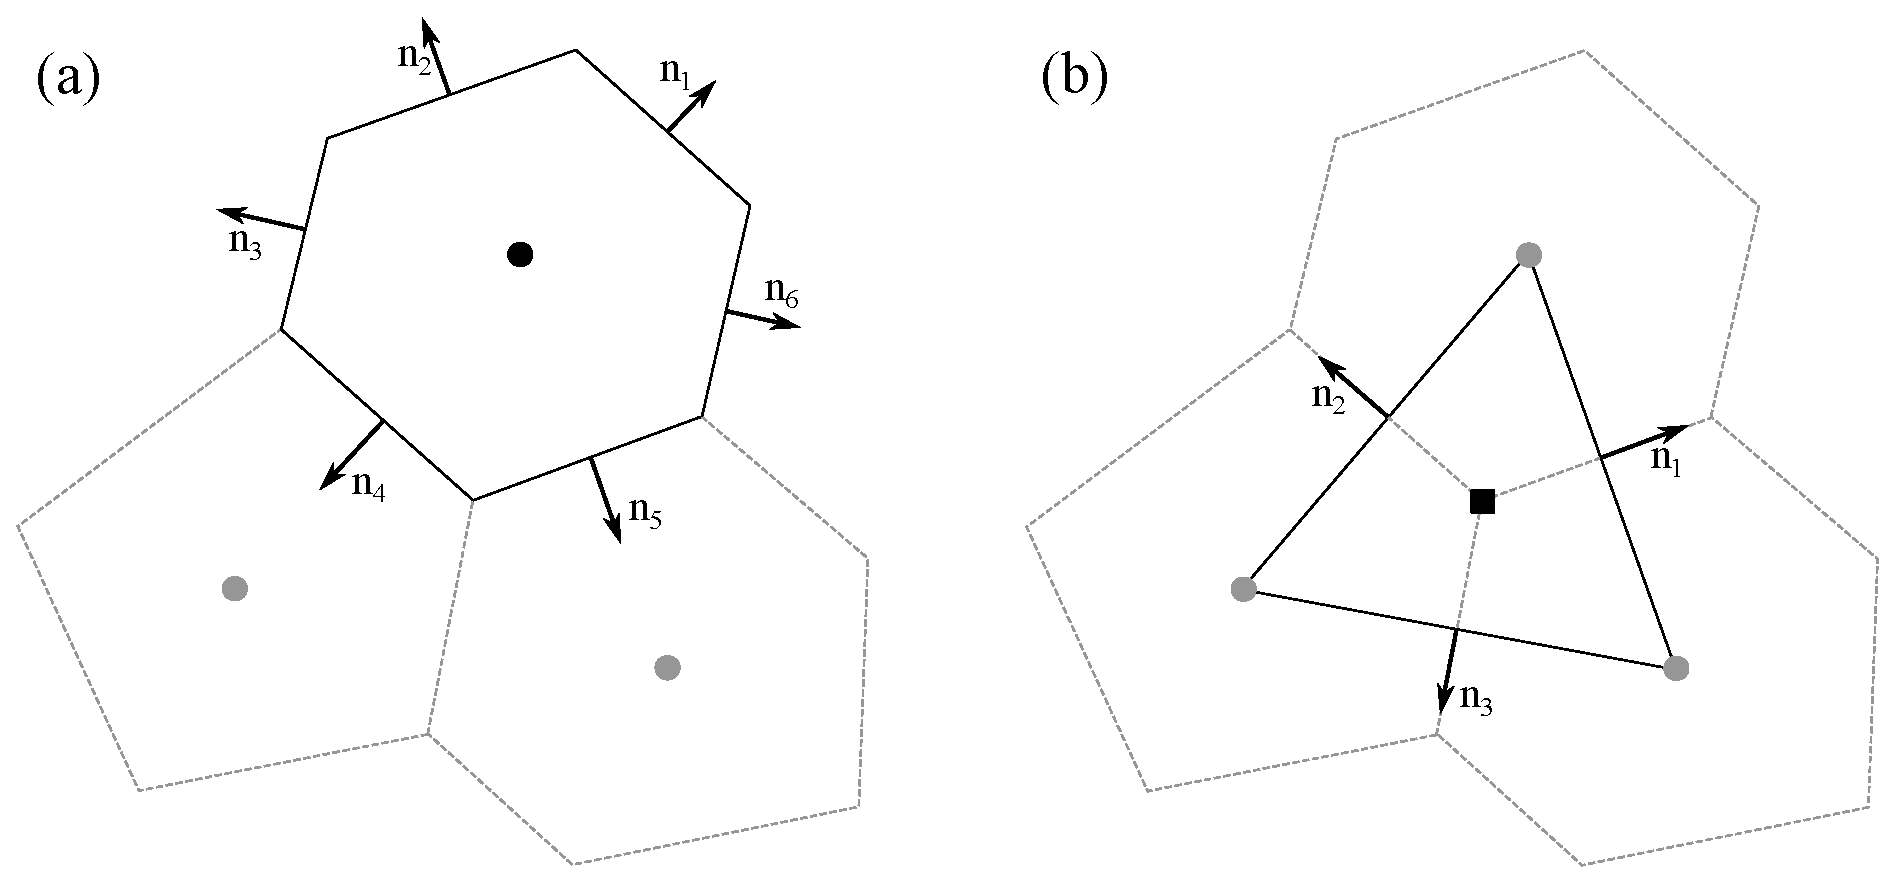
\includegraphics[width=\linewidth]{seaice/figures/mesh_weak.eps}
\caption{Contour integration lines used by the weak scheme. (a): Strain rate at cell centers (\emph{circle}) are calculated from line integrals around primary mesh cells (\emph{solid line}). (b): Divergence of stress at cell vertices (\emph{square}) are calculated from line integrals around the dual mesh cells (\emph{solid line}). Directions of normal vectors used in the integrals are shown for both figures.}
\label{fig:mesh_weak}
\end{figure}

For the weak scheme we use line integrals around cells in the primary and dual meshes to calculate the strain rate tensor and the divergence of stress, respectively. To determine the strain rate tensor we start from the following vector identity:
\begin{equation}
\boldsymbol{\nabla} \cdot (\boldsymbol{u} \otimes \boldsymbol{v}) = (\boldsymbol{u} \cdot \boldsymbol{\nabla}) \boldsymbol{v} + (\boldsymbol{\nabla} \cdot \boldsymbol{u}) \boldsymbol{v}
\label{eqn:vector_identity}
\end{equation}
and from the divergence theorem:
\begin{equation}
\int_\Omega \left[ \boldsymbol{\nabla} \cdot (\boldsymbol{u} \otimes \boldsymbol{v}) \right] \partial{\Omega} = \oint_S \left[\boldsymbol{n} \cdot (\boldsymbol{u} \otimes \boldsymbol{v}) \right] \partial{S} = \oint_S \left[(\boldsymbol{n} \cdot \boldsymbol{u}) \boldsymbol{v} \right] \partial{S}
\label{eqn:divergence_theorem}
\end{equation}
where $\boldsymbol{n}$ is a normal vector to the surface $S$ and $\otimes$ is the tensor product.
If equation \ref{eqn:vector_identity} is integrated over $\Omega$, using equation \ref{eqn:divergence_theorem} we obtain
\begin{equation}
\int_\Omega \left[ (\boldsymbol{u} \cdot \boldsymbol{\nabla}) \boldsymbol{v} + (\boldsymbol{\nabla} \cdot \boldsymbol{u}) \boldsymbol{v} \right] \partial{\Omega} = \oint_S \left[(\boldsymbol{n} \cdot \boldsymbol{u}) \boldsymbol{v} \right] \partial{S}
\label{eqn:weak1}
\end{equation}
If $\boldsymbol{u}$ is chosen as constant then $\boldsymbol{\nabla} \cdot \boldsymbol{u}$ vanishes as does the second term in equation \ref{eqn:weak1}. Taking, also, $\boldsymbol{u}$ sequentially as the cartesian unit vectors spanning $\Omega$ and summing the results we obtain
\begin{equation}
\int_\Omega \left[ \boldsymbol{\nabla} \boldsymbol{v} \right] \partial{\Omega} = \oint_S \left[ \boldsymbol{n} \otimes \boldsymbol{v} \right] \partial{S}
\end{equation}
The symmetric version of this operator is then obtained as:
\begin{equation}
\int_\Omega \left[ \boldsymbol{\nabla_S} \boldsymbol{v} \right] \partial{\Omega} = \oint_S \left[ \boldsymbol{n} \otimes \boldsymbol{v} + \boldsymbol{v} \otimes \boldsymbol{n} \right] \partial{S}
\end{equation}
The strain rate at a point is then obtained from the limit
\begin{equation}
\boldsymbol{\dot{\epsilon}} = \boldsymbol{\nabla}_S \boldsymbol{v} = \lim_{A \to 0} \frac{1}{A} \oint \frac{1}{2}\left[ \boldsymbol{n} \otimes \boldsymbol{v} + \boldsymbol{v} \otimes \boldsymbol{n} \right] \mathrm{d}l
\end{equation}
where the integral is around a closed loop with area $A$ and normal vector $\boldsymbol{n}$, and $\boldsymbol{v}$ is the sea-ice velocity.
To determine the strain rate tensor at the centers of the primary mesh, we take this integration around the edges of the cells in the primary mesh. First the cell is projected onto a flat tangent plane perpendicular to the vector joining the center of the sphere to the cell center. We take the sea ice velocity at a cell edge as the average of the values on the two vertices forming that edge projected onto the tangent plane:
\begin{equation}
\boldsymbol{\dot{\epsilon}}^\prime = \frac{1}{A} \sum_i^{n_e} \frac{1}{2} \left[ \boldsymbol{n}_i \otimes \boldsymbol{v}_i + \boldsymbol{v}_i \otimes \boldsymbol{n}_i \right] l_i
\end{equation}
Here, $A$ is the area of the primary cell, the summation is over the $n_e$ edges of the primary cell, $\boldsymbol{n}_i$ is the normal vector to the edge $i$ that lies in the tangent plane, $\boldsymbol{v}_i$ is the edge velocity and $l_i$ is the length of edge $i$. We use the tangental projection of the velocity and account for metric terms separately. The full strain rate tensor including these metric terms is \citep{Batchelor67}:
\begin{equation}
\dot{\epsilon}_{11} = \dot{\epsilon}_{11}^\prime - \frac{v \tan{\phi}}{r}
\end{equation}
\begin{equation}
\dot{\epsilon}_{22} = \dot{\epsilon}_{22}^\prime
\end{equation}
\begin{equation}
\dot{\epsilon}_{12} = \dot{\epsilon}_{12}^\prime + \frac{u \tan{\phi}}{2r}
\end{equation}
where the prime symbol signifies a strain rate without metric terms.
The stress, which is determined from the strain rate tensor using the constitutive relation, is now defined on cell centers. To find its divergence we use the divergence theorem:
\begin{equation}
\iint \boldsymbol{\nabla} \cdot \boldsymbol{\sigma} \mathrm{d}A = \oint \left[ \boldsymbol{\sigma} \cdot \boldsymbol{n} \right] \mathrm{d}l
\end{equation}
or
\begin{equation}
\boldsymbol{\nabla} \cdot \boldsymbol{\sigma} = \lim_{A \to 0}  \frac{1}{A} \oint \left[ \boldsymbol{\sigma} \cdot \boldsymbol{n} \right] \mathrm{d}l
\end{equation}
for the divergence of stress at a point.
The divergence of internal stress is determined at primary cell vertices (where the velocity is defined and momentum equation solved) by performing a sum around the edges of the dual mesh on a tangent projected plane, tangental to the primary cell vertex. The vertices of the dual mesh are the cell centers of the primary mesh where the strain rate has been determined. The divergence of stress at primary cell vertices is then given by
\begin{equation}
(\boldsymbol{\nabla} \cdot \boldsymbol{\sigma})^\prime = \frac{1}{A_d} \sum_i^{n_c} \left[ \boldsymbol{\sigma}_i \cdot \boldsymbol{n}_i \right] l_i
\end{equation}
where $A_d$ is the area of the dual mesh cell, the sum is over the $n_c$ vertices of the dual mesh, $l_i$ is the length of the $i$ edge of the dual mesh, and $n_i$ is a normal vector to the $i$ edge on the projected plane. As before, this gives a result without taking into account metric effects of the mesh. With those effects the divergence of stress is:
\begin{equation}
(\nabla \cdot \sigma)_u = (\nabla \cdot \sigma)_u^\prime - \frac{2 \sigma_{12} \tan{\phi}}{r}
\end{equation}
\begin{equation}
(\nabla \cdot \sigma)_v = (\nabla \cdot \sigma)_v^\prime + \frac{(\sigma_{11} + \sigma_{22}) \tan{\phi}}{r}
\end{equation}
where the components of $\boldsymbol{\sigma}$ are approximated as the
average of the values on the dual mesh vertices.

\vspace{0.5in}
{\small
\begin{center}
\begin{longtable}{| p{2.0in} || p{4.0in} |}
	\hline
	{\bf Name} & {\bf Description} \endfirsthead
	\hline 
	{\bf Name} & {\bf Description} (Continued) \endhead
	\hline
	\hline
	\hyperref[sec:nm_sec_config_velocity_solver]{config\_velocity\_solver} & Selection of the method for solving ice velocity. \\
	\hline
\end{longtable}
\end{center}
}
\subsection[advection]{advection}
\label{subsec:forward_nm_tab_advection}
The advection namelist record controls options assocated with advection of thickness and tracers.  Tracer advection is not currently supported.

\vspace{0.5in}
{\small
\begin{center}
\begin{longtable}{| p{2.0in} || p{4.0in} |}
	\hline
	{\bf Name} & {\bf Description} \endfirsthead
	\hline 
	{\bf Name} & {\bf Description} (Continued) \endhead
	\hline
	\hline
	\hyperref[sec:nm_sec_config_thickness_advection]{config\_thickness\_advection} & Selection of the method for advecting thickness. \\
	\hline
	\hyperref[sec:nm_sec_config_tracer_advection]{config\_tracer\_advection} & Selection of the method for advecting tracers. \\
	\hline
\end{longtable}
\end{center}
}
\subsection[physical\_parameters]{physical\_parameters}
\label{subsec:forward_nm_tab_physical_parameters}
The physical\_parameters namelist record sets scalar physical parameters and constants within the land ice model.

\vspace{0.5in}
{\small
\begin{center}
\begin{longtable}{| p{2.0in} || p{4.0in} |}
	\hline
	{\bf Name} & {\bf Description} \endfirsthead
	\hline 
	{\bf Name} & {\bf Description} (Continued) \endhead
	\hline
	\hline
	\hyperref[sec:nm_sec_config_ice_density]{config\_ice\_density} & ice density to use \\
	\hline
	\hyperref[sec:nm_sec_config_ocean_density]{config\_ocean\_density} & ocean density to use for calculating floatation \\
	\hline
	\hyperref[sec:nm_sec_config_sea_level]{config\_sea\_level} & sea level to use for calculating floatation \\
	\hline
	\hyperref[sec:nm_sec_config_default_flowParamA]{config\_default\_flowParamA} &  Defines the default value of the flow law parameter A to be used if it is not being calculated from ice temperature.  Defaults to the SI representation of 1.0e-16 yr $^{-1}$  Pa $^{-3}$ . \\
	\hline
	\hyperref[sec:nm_sec_config_flowLawExponent]{config\_flowLawExponent} & Defines the value of the Glen flow law exponent, n. \\
	\hline
	\hyperref[sec:nm_sec_config_dynamic_thickness]{config\_dynamic\_thickness} & Defines the ice thickness below which dynamics are not calculated. \\
	\hline
\end{longtable}
\end{center}
}
\subsection[time\_integration]{time\_integration}
\label{subsec:forward_nm_tab_time_integration}
The time integration namelist controls parameters that pertain to all time-stepping methods.  At present, Forward Euler is the only time integration method implemented.

\vspace{0.5in}
{\small
\begin{center}
\begin{longtable}{| p{2.0in} || p{4.0in} |}
	\hline
	{\bf Name} & {\bf Description} \endfirsthead
	\hline 
	{\bf Name} & {\bf Description} (Continued) \endhead
	\hline
	\hline
	\hyperref[sec:nm_sec_config_dt]{config\_dt} & Length of model time step defined as a time interval. \\
	\hline
	\hyperref[sec:nm_sec_config_time_integration]{config\_time\_integration} & Time integration method. \\
	\hline
\end{longtable}
\end{center}
}
\subsection[time\_management]{time\_management}
\label{subsec:forward_nm_tab_time_management}
General time management is handled by the time\_management namelist record.
Included options handle time-related parts of MPAS, such as the calendar and if the simulation is a restart or not.

Users should use this record to specify the beginning time of the simulation,
and either the duration or the end of the simulation. Only the end or the
duration need to be specified as the other is derived within MPAS from the
beginning time and other specified one.

{\bf TBA: If both duration and stop are specified, then what happens?)}

\vspace{0.5in}
{\small
\begin{center}
\begin{longtable}{| p{2.0in} || p{4.0in} |}
	\hline
	{\bf Name} & {\bf Description} \endfirsthead
	\hline 
	{\bf Name} & {\bf Description} (Continued) \endhead
	\hline
	\hline
	\hyperref[sec:nm_sec_config_do_restart]{config\_do\_restart} & Determines if the initial conditions should be read from a restart file, or an input file.  To perform a restart, simply set this to true in the namelist.input file and modify the start time to be the time you want restart from.  A restart will read the grid information from the input field, and the restart state from the restart file.  It will perform a run normally, except velocity will not be solved on a restart. \\
	\hline
	\hyperref[sec:nm_sec_config_restart_timestamp_name]{config\_restart\_timestamp\_name} & Path to the filename for restart timestamps to be read and written from. \\
	\hline
	\hyperref[sec:nm_sec_config_start_time]{config\_start\_time} & Timestamp describing the initial time of the simulation.  If it is set to 'file', the initial time is read from restart\_timestamp \\
	\hline
	\hyperref[sec:nm_sec_config_stop_time]{config\_stop\_time} & Timestamp describing the final time of the simulation. If it is set to 'none' the final time is determined from config\_start\_time and config\_run\_duration.  If config\_run\_duration is also specified, it takes precedence over config\_stop\_time.  Set config\_stop\_time to be equal to config\_start\_time (and config\_run\_duration to 'none') to perform a diagnostic solve only. \\
	\hline
	\hyperref[sec:nm_sec_config_run_duration]{config\_run\_duration} & Timestamp describing the length of the simulation. If it is set to 'none' the duration is determined from config\_start\_time and config\_stop\_time. config\_run\_duration overrides inconsistent values of config\_stop\_time. If a time value is specified for config\_run\_duration, it must be greater than 0. \\
	\hline
	\hyperref[sec:nm_sec_config_calendar_type]{config\_calendar\_type} & Selection of the type of calendar that should be used in the simulation. \\
	\hline
\end{longtable}
\end{center}
}
\subsection[io]{io}
\label{subsec:forward_nm_tab_io}
The io namelist record provides options for modifications to the I/O system of
MPAS. These include frequency, file name, and parallelization options.

\vspace{0.5in}
{\small
\begin{center}
\begin{longtable}{| p{2.0in} || p{4.0in} |}
	\hline
	{\bf Name} & {\bf Description} \endfirsthead
	\hline 
	{\bf Name} & {\bf Description} (Continued) \endhead
	\hline
	\hline
	\hyperref[sec:nm_sec_config_write_output_on_startup]{config\_write\_output\_on\_startu-}\hyperref[sec:nm_sec_config_write_output_on_startup]{p}& Logical flag determining if an output file should be written prior to the first time step. \\
	\hline
	\hyperref[sec:nm_sec_config_pio_num_iotasks]{config\_pio\_num\_iotasks} & Integer specifying how many IO tasks should be used within the PIO library. A value of 0 causes all MPI tasks to also be IO tasks. IO tasks are required to write contiguous blocks of data to a file. \\
	\hline
	\hyperref[sec:nm_sec_config_pio_stride]{config\_pio\_stride} & Integer specifying the stride of each IO task. \\
	\hline
	\hyperref[sec:nm_sec_config_year_digits]{config\_year\_digits} & Integer specifying the number of digits used to represent the year in time strings. \\
	\hline
\end{longtable}
\end{center}
}
\subsection[decomposition]{decomposition}
\label{subsec:forward_nm_tab_decomposition}
MPAS handles decomposing all variables into computational blocks. The
decomposition used needs to be specified at run time and is computed by an
external tool (e.g. metis). Additionally, MPAS supports multiple computational
blocks per MPI process, and the user may specify an additional decomposition
file which can specify the assignment of blocks to MPI processes. Run-time
parameters that control the run-time decomposition used are specified within
the decomposition namelist record.


\vspace{0.5in}
{\small
\begin{center}
\begin{longtable}{| p{2.0in} || p{4.0in} |}
	\hline
	{\bf Name} & {\bf Description} \endfirsthead
	\hline 
	{\bf Name} & {\bf Description} (Continued) \endhead
	\hline
	\hline
	\hyperref[sec:nm_sec_config_num_halos]{config\_num\_halos} & Determines the number of halo cells extending from a blocks owned cells (Called the 0-Halo). The default of 3 is the minimum that can be used with monotonic advection. \\
	\hline
	\hyperref[sec:nm_sec_config_block_decomp_file_prefix]{config\_block\_decomp\_file\_prefix} & Defines the prefix for the block decomposition file. Can include a path. The number of blocks is appended to the end of the prefix at run-time. \\
	\hline
	\hyperref[sec:nm_sec_config_number_of_blocks]{config\_number\_of\_blocks} & Determines the number of blocks a simulation should be run with. If it is set to 0, the number of blocks is the same as the number of MPI tasks at run-time. \\
	\hline
	\hyperref[sec:nm_sec_config_explicit_proc_decomp]{config\_explicit\_proc\_decomp} & Determines if an explicit processor decomposition should be used. This is only useful if multiple blocks per processor are used. \\
	\hline
	\hyperref[sec:nm_sec_config_proc_decomp_file_prefix]{config\_proc\_decomp\_file\_prefix} & Defines the prefix for the processor decomposition file. This file is only read if config\_explicit\_proc\_decomp is .true. The number of processors is appended to the end of the prefix at run-time. \\
	\hline
\end{longtable}
\end{center}
}
\subsection[debug]{debug}
\label{subsec:forward_nm_tab_debug}
At run-time a user can enable debugging features within MPAS-Ocean. These
features include disabling any tendencies to help determine why an issue might
be happening. Debugging options also include various checks on certain fields,
and the ability to prescribe both a thickness and velocity field at run-time
which are constant throughout a simulation. All options that control these
debugging features are specified within the debug namelist record.

\vspace{0.5in}
{\small
\begin{center}
\begin{longtable}{| p{2.0in} || p{4.0in} |}
	\hline
	{\bf Name} & {\bf Description} \endfirsthead
	\hline 
	{\bf Name} & {\bf Description} (Continued) \endhead
	\hline
	\hline
	\hyperref[sec:nm_sec_config_print_thickness_advection_info]{config\_print\_thickness\_advectio-}\hyperref[sec:nm_sec_config_print_thickness_advection_info]{n\_info}& Prints additional information about thickness advection. \\
	\hline
\end{longtable}
\end{center}
}
\section[Variable definitions]{\hyperref[chap:variable_sections]{Variable definitions}}
\label{sec:forward_variable_tables}
Embedded links point to more detailed variable information in the appendix.
\subsection[state]{\hyperref[sec:var_sec_state]{state}}
\label{subsec:forward_var_tab_state}
\vspace{0.5in}
{\small
\begin{center}
\begin{longtable}{| p{2.0in} | p{4.0in} |}
	\hline
	{\bf Name} & {\bf Description} \endfirsthead
	\hline 
	{\bf Name} & {\bf Description} (Continued) \endhead
	\hline
	\hyperref[subsec:var_sec_state_xtime]{xtime} & model time, with format 'YYYY-MM-DD\_HH:MM:SS' \\
	\hline
	\hyperref[subsec:var_sec_state_thickness]{thickness} & ice thickness \\
	\hline
	\hyperref[subsec:var_sec_state_layerThickness]{layerThickness} & layer thickness \\
	\hline
	\hyperref[subsec:var_sec_state_temperature]{temperature} & ice temperature \\
	\hline
	\hyperref[subsec:var_sec_state_lowerSurface]{lowerSurface} & elevation at bottom of ice \\
	\hline
	\hyperref[subsec:var_sec_state_upperSurface]{upperSurface} & elevation at top of ice \\
	\hline
	\hyperref[subsec:var_sec_state_layerThicknessEdge]{layerThicknessEdge} & layer thickness on cell edges \\
	\hline
	\hyperref[subsec:var_sec_state_upperSurfaceVertex]{upperSurfaceVertex} & elevation at top of ice on vertices (currently only needed by shallow ice solver) \\
	\hline
	\hyperref[subsec:var_sec_state_cellMask]{cellMask} & bitmask indicating various properties about the ice sheet on cells.  cellMask only needs to be a restart field if config\_allow\_additional\_advance = false (to keep the mask of initial ice extent) \\
	\hline
	\hyperref[subsec:var_sec_state_edgeMask]{edgeMask} & bitmask indicating various properties about the ice sheet on edges. \\
	\hline
	\hyperref[subsec:var_sec_state_vertexMask]{vertexMask} & bitmask indicating various properties about the ice sheet on vertices. \\
	\hline
	\hyperref[subsec:var_sec_state_normalVelocity]{normalVelocity} & horizonal velocity, normal component to an edge \\
	\hline
	\hyperref[subsec:var_sec_state_uReconstructX]{uReconstructX} & x-component of velocity reconstructed on cell centers \\
	\hline
	\hyperref[subsec:var_sec_state_uReconstructY]{uReconstructY} & y-component of velocity reconstructed on cell centers \\
	\hline
	\hyperref[subsec:var_sec_state_uReconstructZ]{uReconstructZ} & z-component of velocity reconstructed on cell centers \\
	\hline
	\hyperref[subsec:var_sec_state_uReconstructZonal]{uReconstructZonal} & zonal velocity reconstructed on cell centers \\
	\hline
	\hyperref[subsec:var_sec_state_uReconstructMeridional]{uReconstructMeridional} & meridional velocity reconstructed on cell centers \\
	\hline
\end{longtable}
\end{center}
}
\subsection[tend]{\hyperref[sec:var_sec_tend]{tend}}
\label{subsec:forward_var_tab_tend}
\vspace{0.5in}
{\small
\begin{center}
\begin{longtable}{| p{2.0in} | p{4.0in} |}
	\hline
	{\bf Name} & {\bf Description} \endfirsthead
	\hline 
	{\bf Name} & {\bf Description} (Continued) \endhead
	\hline
	\hyperref[subsec:var_sec_tend_tend_layerThickness]{tend\_layerThickness} & time tendency of layer thickness \\
	\hline
	\hyperref[subsec:var_sec_tend_tend_temperature]{tend\_temperature} & time tendency of ice temperature \\
	\hline
\end{longtable}
\end{center}
}
\subsection[mesh]{\hyperref[sec:var_sec_mesh]{mesh}}
\label{subsec:forward_var_tab_mesh}
\vspace{0.5in}
{\small
\begin{center}
\begin{longtable}{| p{2.0in} | p{4.0in} |}
	\hline
	{\bf Name} & {\bf Description} \endfirsthead
	\hline 
	{\bf Name} & {\bf Description} (Continued) \endhead
	\hline
	\hyperref[subsec:var_sec_mesh_latCell]{latCell} & Latitude location of cell centers in radians. \\
	\hline
	\hyperref[subsec:var_sec_mesh_lonCell]{lonCell} & Longitude location of cell centers in radians. \\
	\hline
	\hyperref[subsec:var_sec_mesh_xCell]{xCell} & X Coordinate in cartesian space of cell centers. \\
	\hline
	\hyperref[subsec:var_sec_mesh_yCell]{yCell} & Y Coordinate in cartesian space of cell centers. \\
	\hline
	\hyperref[subsec:var_sec_mesh_zCell]{zCell} & Z Coordinate in cartesian space of cell centers. \\
	\hline
	\hyperref[subsec:var_sec_mesh_indexToCellID]{indexToCellID} & List of global cell IDs. \\
	\hline
	\hyperref[subsec:var_sec_mesh_latEdge]{latEdge} & Latitude location of edge midpoints in radians. \\
	\hline
	\hyperref[subsec:var_sec_mesh_lonEdge]{lonEdge} & Longitude location of edge midpoints in radians. \\
	\hline
	\hyperref[subsec:var_sec_mesh_xEdge]{xEdge} & X Coordinate in cartesian space of edge midpoints. \\
	\hline
	\hyperref[subsec:var_sec_mesh_yEdge]{yEdge} & Y Coordinate in cartesian space of edge midpoints. \\
	\hline
	\hyperref[subsec:var_sec_mesh_zEdge]{zEdge} & Z Coordinate in cartesian space of edge midpoints. \\
	\hline
	\hyperref[subsec:var_sec_mesh_indexToEdgeID]{indexToEdgeID} & List of global edge IDs. \\
	\hline
	\hyperref[subsec:var_sec_mesh_latVertex]{latVertex} & Latitude location of vertices in radians. \\
	\hline
	\hyperref[subsec:var_sec_mesh_lonVertex]{lonVertex} & Longitude location of vertices in radians. \\
	\hline
	\hyperref[subsec:var_sec_mesh_xVertex]{xVertex} & X Coordinate in cartesian space of vertices. \\
	\hline
	\hyperref[subsec:var_sec_mesh_yVertex]{yVertex} & Y Coordinate in cartesian space of vertices. \\
	\hline
	\hyperref[subsec:var_sec_mesh_zVertex]{zVertex} & Z Coordinate in cartesian space of vertices. \\
	\hline
	\hyperref[subsec:var_sec_mesh_indexToVertexID]{indexToVertexID} & List of global vertex IDs. \\
	\hline
	\hyperref[subsec:var_sec_mesh_cellsOnEdge]{cellsOnEdge} & List of cells that straddle each edge. \\
	\hline
	\hyperref[subsec:var_sec_mesh_nEdgesOnCell]{nEdgesOnCell} & Number of edges that border each cell. \\
	\hline
	\hyperref[subsec:var_sec_mesh_nEdgesOnEdge]{nEdgesOnEdge} & Number of edges that surround each of the cells that straddle each edge. These edges are used to reconstruct the tangential velocities. \\
	\hline
	\hyperref[subsec:var_sec_mesh_edgesOnCell]{edgesOnCell} & List of edges that border each cell. \\
	\hline
	\hyperref[subsec:var_sec_mesh_edgesOnEdge]{edgesOnEdge} & List of edges that border each of the cells that straddle each edge. \\
	\hline
	\hyperref[subsec:var_sec_mesh_weightsOnEdge]{weightsOnEdge} & Reconstruction weights associated with each of the edgesOnEdge. \\
	\hline
	\hyperref[subsec:var_sec_mesh_dvEdge]{dvEdge} & Length of each edge, computed as the distance between verticesOnEdge. \\
	\hline
	\hyperref[subsec:var_sec_mesh_dcEdge]{dcEdge} & Length of each edge, computed as the distance between cellsOnEdge. \\
	\hline
	\hyperref[subsec:var_sec_mesh_angleEdge]{angleEdge} & Angle the edge normal makes with local eastward direction. \\
	\hline
	\hyperref[subsec:var_sec_mesh_areaCell]{areaCell} & Area of each cell in the primary grid. \\
	\hline
	\hyperref[subsec:var_sec_mesh_areaTriangle]{areaTriangle} & Area of each cell (triangle) in the dual grid. \\
	\hline
	\hyperref[subsec:var_sec_mesh_edgeNormalVectors]{edgeNormalVectors} & Normal vector defined at an edge. \\
	\hline
	\hyperref[subsec:var_sec_mesh_localVerticalUnitVectors]{localVerticalUnitVectors} & Unit surface normal vectors defined at cell centers. \\
	\hline
	\hyperref[subsec:var_sec_mesh_cellTangentPlane]{cellTangentPlane} & The two vectors that define a tangent plane at a cell center. \\
	\hline
	\hyperref[subsec:var_sec_mesh_cellsOnCell]{cellsOnCell} & List of cells that neighbor each cell. \\
	\hline
	\hyperref[subsec:var_sec_mesh_verticesOnCell]{verticesOnCell} & List of vertices that border each cell. \\
	\hline
	\hyperref[subsec:var_sec_mesh_verticesOnEdge]{verticesOnEdge} & List of vertices that straddle each edge. \\
	\hline
	\hyperref[subsec:var_sec_mesh_edgesOnVertex]{edgesOnVertex} & List of edges that share a vertex as an endpoint. \\
	\hline
	\hyperref[subsec:var_sec_mesh_cellsOnVertex]{cellsOnVertex} & List of cells that share a vertex. \\
	\hline
	\hyperref[subsec:var_sec_mesh_kiteAreasOnVertex]{kiteAreasOnVertex} & Area of the portions of each dual cell that are part of each cellsOnVertex. \\
	\hline
	\hyperref[subsec:var_sec_mesh_coeffs_reconstruct]{coeffs\_reconstruct} & Coefficients to reconstruct velocity vectors at cells centers. \\
	\hline
	\hyperref[subsec:var_sec_mesh_edgeSignOnCell]{edgeSignOnCell} & Sign of edge contributions to a cell for each edge on cell. Used for bit-reproducible loops. Represents directionality of vector connecting cells. \\
	\hline
	\hyperref[subsec:var_sec_mesh_edgeSignOnVertex]{edgeSignOnVertex} & Sign of edge contributions to a vertex for each edge on vertex. Used for bit-reproducible loops. Represents directionality of vector connecting vertices. \\
	\hline
	\hyperref[subsec:var_sec_mesh_layerThicknessFractions]{layerThicknessFractions} & Fractional thickness of each sigma layer \\
	\hline
	\hyperref[subsec:var_sec_mesh_layerCenterSigma]{layerCenterSigma} & Sigma (fractional) level at center of each layer \\
	\hline
	\hyperref[subsec:var_sec_mesh_layerInterfaceSigma]{layerInterfaceSigma} & Sigma (fractional) level at interface between each layer (including top and bottom) \\
	\hline
	\hyperref[subsec:var_sec_mesh_bedTopography]{bedTopography} & Elevation of ice sheet bed.  Once isostasy is added to the model, this should become a state variable. \\
	\hline
	\hyperref[subsec:var_sec_mesh_sfcMassBal]{sfcMassBal} & Surface mass balance \\
	\hline
\end{longtable}
\end{center}
}
